\chapter{Atmosniffer Overview} %\label{Atmosniffer Overview}
%\vspace{-7mm}
%\bigskip
This Chapter provides an overview of the device the resarch team at Weber State University, led by Dr. Sohl and Dr. Valle started working on, the AtmoSniffer.

\section{Motivation}

\subsection{Why build a device that can "Sniff" the atmosphore?}
- “An estimated 4.2 million premature deaths globally are linked to ambient air pollution” according to the World Health Organization (WHO). In other words, the equivalent to the entire population of Utah every 9 months dies prematurely because of bad air. WHO estimates that 91\% of the world’s population is living in places where air quality guidelines are not met. Measuring this pollution is the first step in understanding and solving the problem. 


\begin{itemize}
\item \textbf{Problem:}
	\begin{itemize}
	\item Current air monitoring systems can be very large, heavy, and/or expensive
	\item They posses a limited range of sensors typically measuring only one gas type
	\item Are only usable for a specific task or deployment
	\item Require significant AC power.
	\end{itemize}

\item \textbf{Solution:}
	\begin{itemize}
	\item The AtmoSniffer is small and light.
	\item Detects a variety of gas types.
	\item Multiple user interfaces that can be easily accessed.
	\end{itemize}

\end{itemize}

\subsection{AtmoSniffer Project}
\begin{itemize}
\item The research team at Weber State University, led by Dr. Sohl and Dr. Valle started working on a device which is capable of moving air particles through gas sensors and transmit its data through radio and Bluetooth signals to monitor air quality and measure pollution.

\item The current AtmoSniffer prototype, version 0.3, detects CO, CO2, NO, NO2, SO2, NH3, O3, VOCs, fine particulate material (in six size ranges covering 0.3 µm to 10 µm diameter aerosols), temperature, pressure, relative humidity, and inertial/true position. As a complete environmental monitor, turbulence/vibration is detected through a 9-axis inertial sensor.

\item The AtmoSniffer can be deployed as a portable emissions locator or as a long duration air quality monitor staged on a work bench or mounted to pretty much anything.
\end{itemize}

\subsection{AtmoSniffer Device Pictures}
Here are a couple of pictures showing you how the physical device looks like:

\begin{figure}[h]
\centering
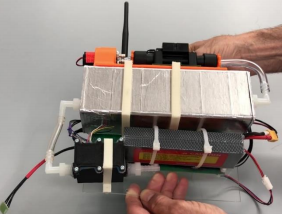
\includegraphics{full_device_cover.png}
 \caption{AtmoSniffer Device Encased, this is how the whole device looks when its assembled.}
 \label{fig:encased_device}
\end{figure}

\begin{figure}[h]
\centering
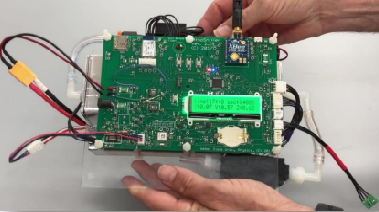
\includegraphics{full_device_nocover.png}
 \caption{Inside AtmoSniffer Device}
 \label{fig:inside_device}
\end{figure}

\begin{figure}[h]
\centering
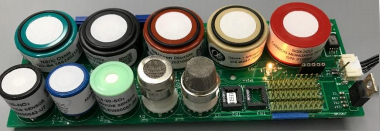
\includegraphics{gas_module.png}
 \caption{This is the Gas Sensors Module, this can be taken on/off like any other module.}
 \label{fig:gas_sensors}
\end{figure}

\begin{figure}[h]
\centering
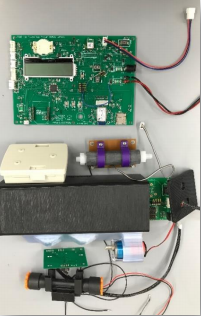
\includegraphics{modules_separated.png}
 \caption{Device Modules}
 \label{fig:device_modules}
\end{figure}

\newpage \subsection{Project Interaces}
\begin{itemize}
\item The device transmits a stream of data via the following communication protocols:
	\begin{itemize}
	\item Xbee radio via UART channel; Fully functional
	\item Bluetooth via UART channel: Fully functional
	\item WIFI via UART Channel: To be develop
	\end{itemize}
\item Supports two Atmosniffer interfaces
	\begin{itemize}
	\item Android App
		\begin{itemize}
		\item Quick Diagnostic
		\item Data Calibration
		\end{itemize}
	\item Desktop Application
		\begin{itemize}
		\item Full Data Analysis
		\item Data Calibration
		\end{itemize}
	\end{itemize}
\end{itemize}
